\documentclass[12pt,a4paper,twoside]{article}
\usepackage{labor}
\begin{document}

%fill for cover and header creation
\newcommand\laboratorynumber{2}
\title{3D Kino/Polarisation}
\newcommand\supervisor{Ditlbacher, Harald}
\newcommand\groupnumber{42}

\newcommand\participantonelastname{Eisner}
\newcommand\participantonefirstname{Nico}
\newcommand\participantoneid{12214121}
\newcommand\participanttwolastname{Waldl}
\newcommand\participanttwofirstname{Philip}
\newcommand\participanttwoid{12214120}
\author{\participantonelastname \ \& \participanttwolastname}

\newcommand\degreeid{UB 033 678}
\newcommand\semester{23WS}
\date{21.10.2023}

%select correct course title
%\newcommand\coursetitle{Einführung in die \\ physikalischen Messmethoden}
%\newcommand\coursetitle{Laborübungen 1: \\ Mechanik und Wärme}
\newcommand\coursetitle{Laborübungen 2: \\ Elektrizität, Magnetismus, Optik}
%\newcommand\coursetitle{Fortgeschrittenen Praktikum 1: \\ Technische Physik}
%\newcommand\coursetitle{Fortgeschrittenen Praktikum 2: \\ Allgemeine Physik}

%\begin{titlepage}
   \begin{center}
       \begin{figure}[H]
            \begin{minipage}[h]{30mm}
                \centerline{
\includegraphics[height=15mm]{cover_nudes/tugraz.png}}
            \end{minipage}
            \hfill
            \begin{minipage}[h]{30mm}
                \centerline{
\includegraphics[height=15mm]{cover_nudes/nawi_graz.png}}
            \end{minipage}
            \hfill
            \begin{minipage}[h]{30mm}
                \centerline{
\includegraphics[height=15mm]{cover_nudes/uni-graz.png}}
            \end{minipage}
        \end{figure}
        
        \large{\emph{Institut für Experimentalphysik der Technischen Universität Graz \\
        \& Institut für Physik der Universität Graz}} \\
        \vspace{5mm}
        
        {\Huge \textbf{\coursetitle}}
        \vspace{5mm}
        
        {\huge \laboratorynumber: \thetitle}
    \end{center}
    
    \vfill
    
    \begin{table}[H]
        \LARGE
        \centering
        \begin{tabular}{r l}
            Betreuer:       & \supervisor \\
            Gruppennummer:  & \groupnumber \\
            \\
            Name:           & \participantonelastname, \participantonefirstname \\
            Matrikelnummer: & \participantoneid \\
            Name:           & \participanttwolastname, \participanttwofirstname \\
            Matrikelnummer: & \participanttwoid \\
            \\
            Kennzahl:       & \degreeid \\
            Datum:          & \semester \ | \thedate
        \end{tabular}
    \end{table}
    \vspace{4cm}
\end{titlepage}
\clearpage
\setcounter{page}{1}

%\maketitle %short title alternative

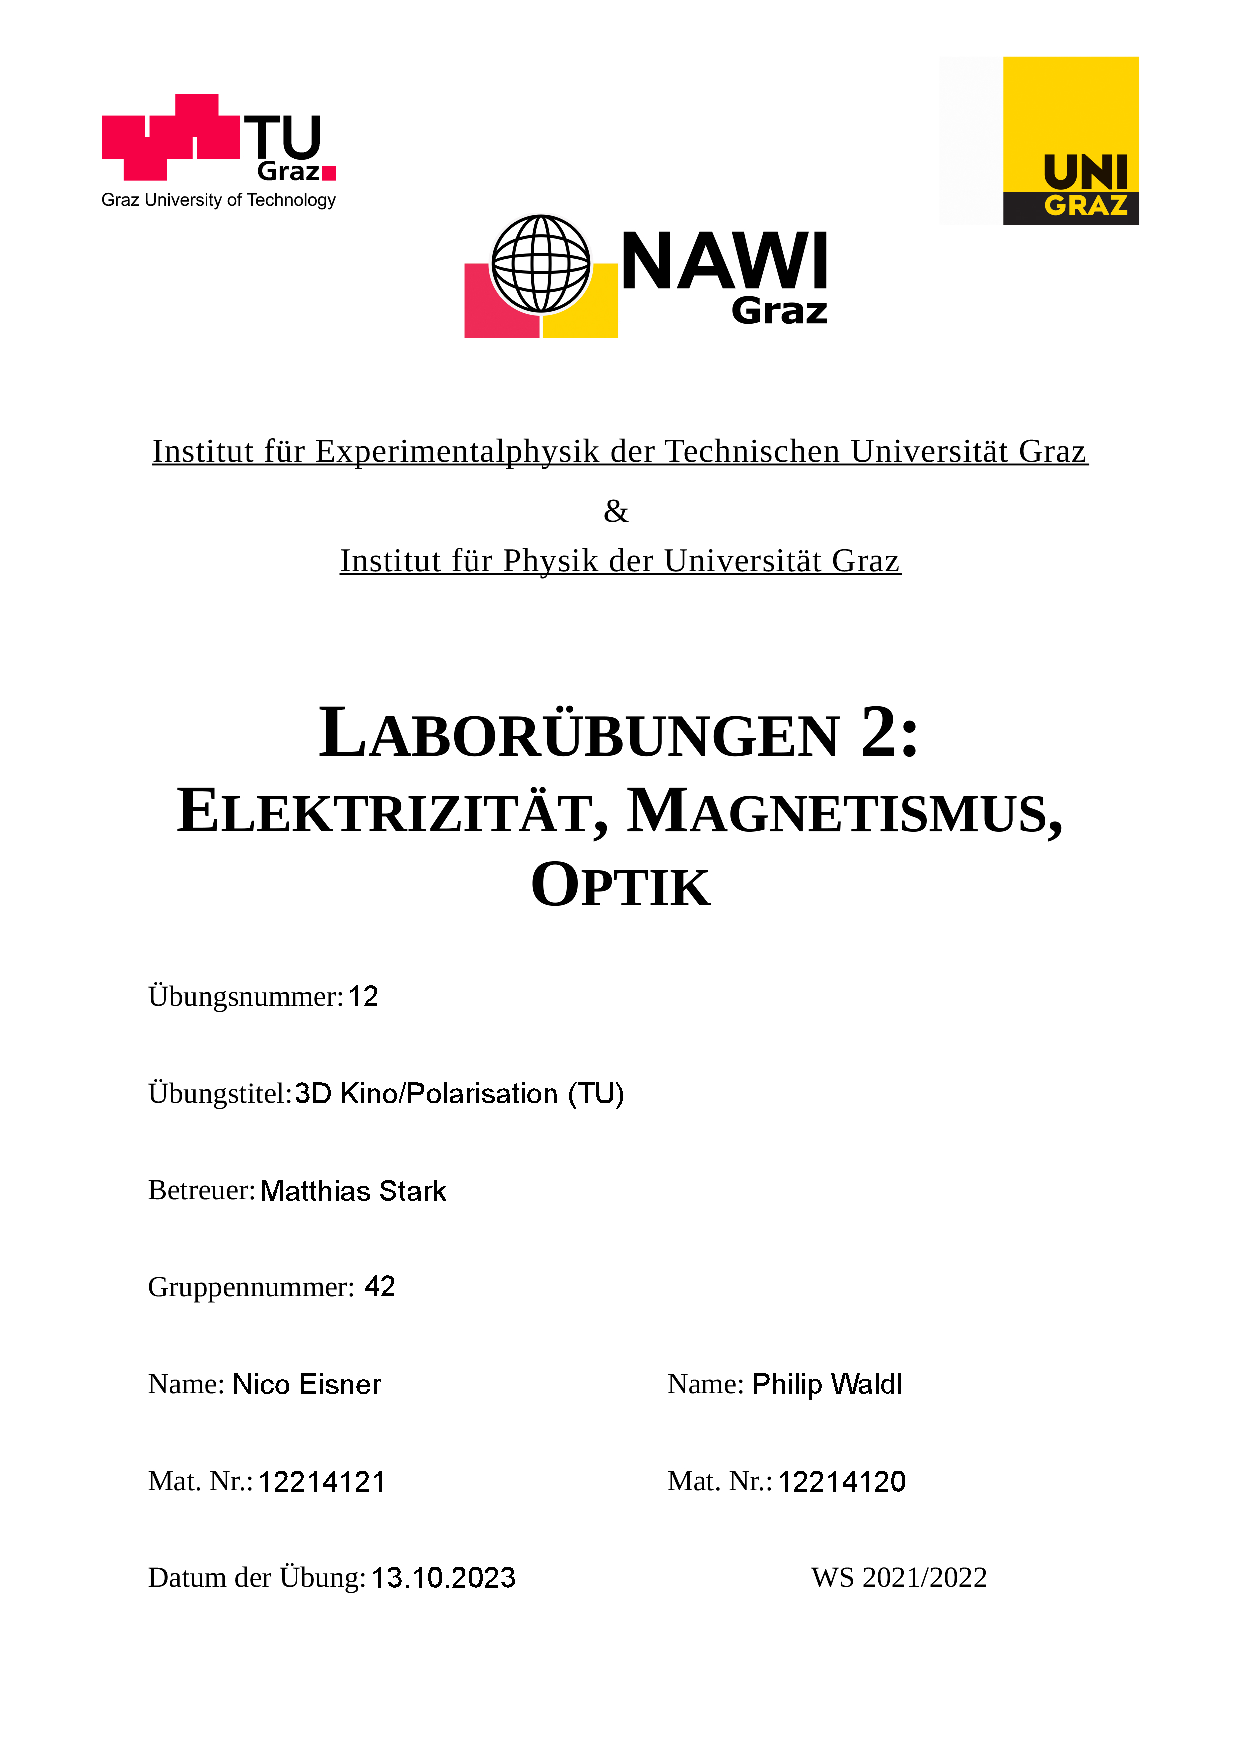
\includepdf[pages={1}]{../Deckblätter/Deckblatt_3DKino.pdf}

\tableofcontents
\newpage

\section{Aufgabenstellung} %jo beschreibn wos gmocht host ------------------------------
Das Experiment 3D Kino/Polarisation besteht aus folgenden Aufgaben. 
Im ersten Teil gilt es das Gesetz von Malus zu beweisen. 
Die Aufgabe im zweiten Teil ist es, die konzentration einer Zuckerlösung zu bestimmen. 
Anschließend wird mithilfe eines Handybildschirmes Spannungsdoppelbrechungen beobachtet. 
\\
Im Teil 3D Kino wird zuerst die Orientierung der Polarisator Folien einer 3D Brille bestimmt. 
Anschließend wird eine 3D Projektion mit dem RealD-verfahren erzeugt. 
\\
\\
Alle Informationen und Methodiken wurden uns von der Technischen Universität bereitgestellt \cite{teachcenter2}. 


\section{Voraussetzungen \& Grundlagen} %Grundlagen erklären, Formeln mit erklärung
Um das Gesetz von Malus zu beweisen, gilt es erst einmal dieses zu kennen. 


    \begin{equation}
        \label{eq:Gesetz von Malus}
        \centerline{$I = I_0 cos^2(\theta) = \vert E_0 \vert ^2 cos^2(\theta)$}
    \end{equation}

\noindent
Eine linear polarisierte Lichtwelle trifft auf einen Polarisator. Dabei ändert sich je nach Winkel $\theta$, unter dem das Licht auf den Polarisator fällt, die Intensität $I$. 
Dabei ist $I_0$ die Intensität des Lichtes vor Durchtritt des Polarisators. 
\\
Der Vektor wird in seine Komponenten zerlegt und parallel und senkrecht in Durchlassrichtung des Polarisators verschoben. 

\begin{figure}[H]
    \centering
    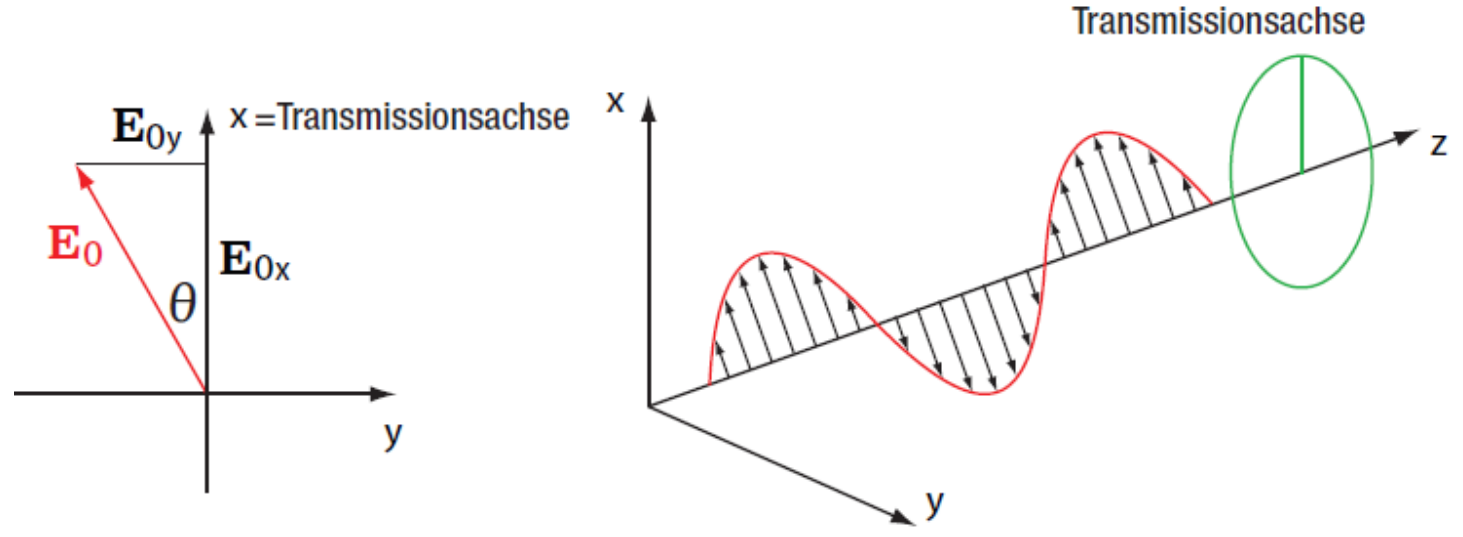
\includegraphics[width=0.6\linewidth]{nudes/Mallus.png}
    \caption{Aufteilung des Vektors einer linear polarisierten Lichtwelle durch den Polarisator. \\ Entnommmen aus Seite 3 Skriptum Polarisation \cite{teachcenter2}}
    \label{fig:Mallus Vektor}
\end{figure}

\noindent
Um die Konzentration der Zuckerlösung zu berechnen benötigt man die Länge des Zuckergefäßes, sowie den Winkel $\varphi$. Die Konzentration $c$ entspricht der stärke der Zuckerlösung. 

\begin{equation}
    \label{eq:Konzentration Zucker}
    \centerline{$\varphi = \varphi_0 cL$}
\end{equation}

\noindent
Die Zuckerlösung dreht die Polarisationsrichtung des Lichtes, da die Zuckermoleküle einen Drehsinn zeigen. 
Daraus folgt, zirkular polarisiertes Licht wird anders transmittiert. 
\\
\\
Durch Druck auf isotropische Materialien lässt sich ein Effekt hervorrufen, bei dem Licht je nach Ausbreitungsrichtung unterschiedlich transmittiert wird. Daraus folgen unterschiedliche Brechungsindizes. 
Übt man Druck auf ein Plastikteil aus, so erkennt man eine unterschiedliche Verspannung im Material, bzw einen unterschiedlichen Brechungsindex. 
Durch einen Polarisator kann dieser Effekt sichtbar gemacht werden. 
\\
\\
Einen 3D Effekt erzeugt man, indem man aus zwei verschiedenen Perspektiven aufgenommene Bilder überlagert und in die Augen des Betrachters leitet. 
Dabei ist jedoch wichtig, dass jeweils nur ein Bild in ein Auge fallen darf, um einen Tiefeneindruck zu erschaffen. 
Das gängigste Verfahren ist das RealD-Verfahren. Hierbei werden vor dem Projektor ein linearer Polarisator und ein $\lambda/4$ (Lambda viertel) Plättchen gestellt. 
Mit den richtigen Einstellungen erhält man für die Lichtwege rechtszirkulierte und für den anderen Weg linkszirkulierte Polarisation. \\
Die 3D-Brille reversiert den Prozess. Dort polarisert ein $\lambda/4$ Plättchen das Licht und trifft dann erneut auf einen Polarisator. 

\begin{figure}[H]
    \centering
    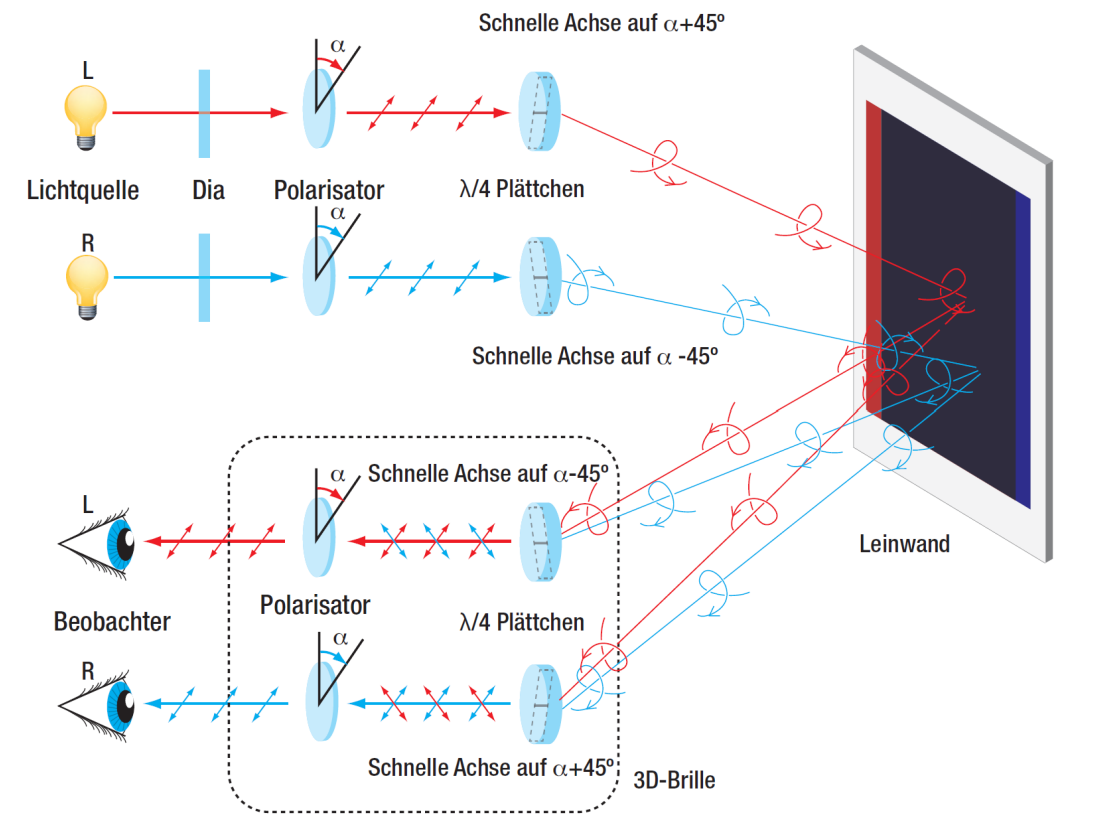
\includegraphics[width=0.6\linewidth]{nudes/3D.png}
    \caption{Darstellung einer 3D Projektion \\ Entnommmen aus Seite 5 Skriptum Polarisation \cite{teachcenter2}}
    \label{fig:3D Projektion schema}
\end{figure}

\noindent
Für die berechnung des Mittelwertes $\bar{\varphi}$, benötigt man die Anzahl der Messversuche N sowie die einzelnen Winkel $\varphi$. 

\begin{equation}
    \label{eq:Mittelwert}
    \centerline{$\bar{\varphi} = \frac{1}{N} \sum_{i = 1}^{N} \varphi_i $} 
\end{equation}

\noindent
Mit dem nun bekannten Mittelwert $\bar{\varphi}$ lässt sich die Standardabweichung $\sigma_{\varphi}$ berechnen. 

\begin{equation}
    \label{eq:Standardabweichung}
    \centerline{$\sigma_{\varphi} = \sqrt{\frac{1}{N-1} \sum_{i = 1}^{N} (\varphi_i - \bar{\varphi})^2}$} 
\end{equation}

\section{Versuchsanordnung} %mit skizze kurz beschreiben ------------------------------
Der Versuch besteht aus verschiedenen Aufbauten. Für den ersten Teil sieht der Versuch wiefolgt aus. 

    \begin{figure}[H]
        \centering
        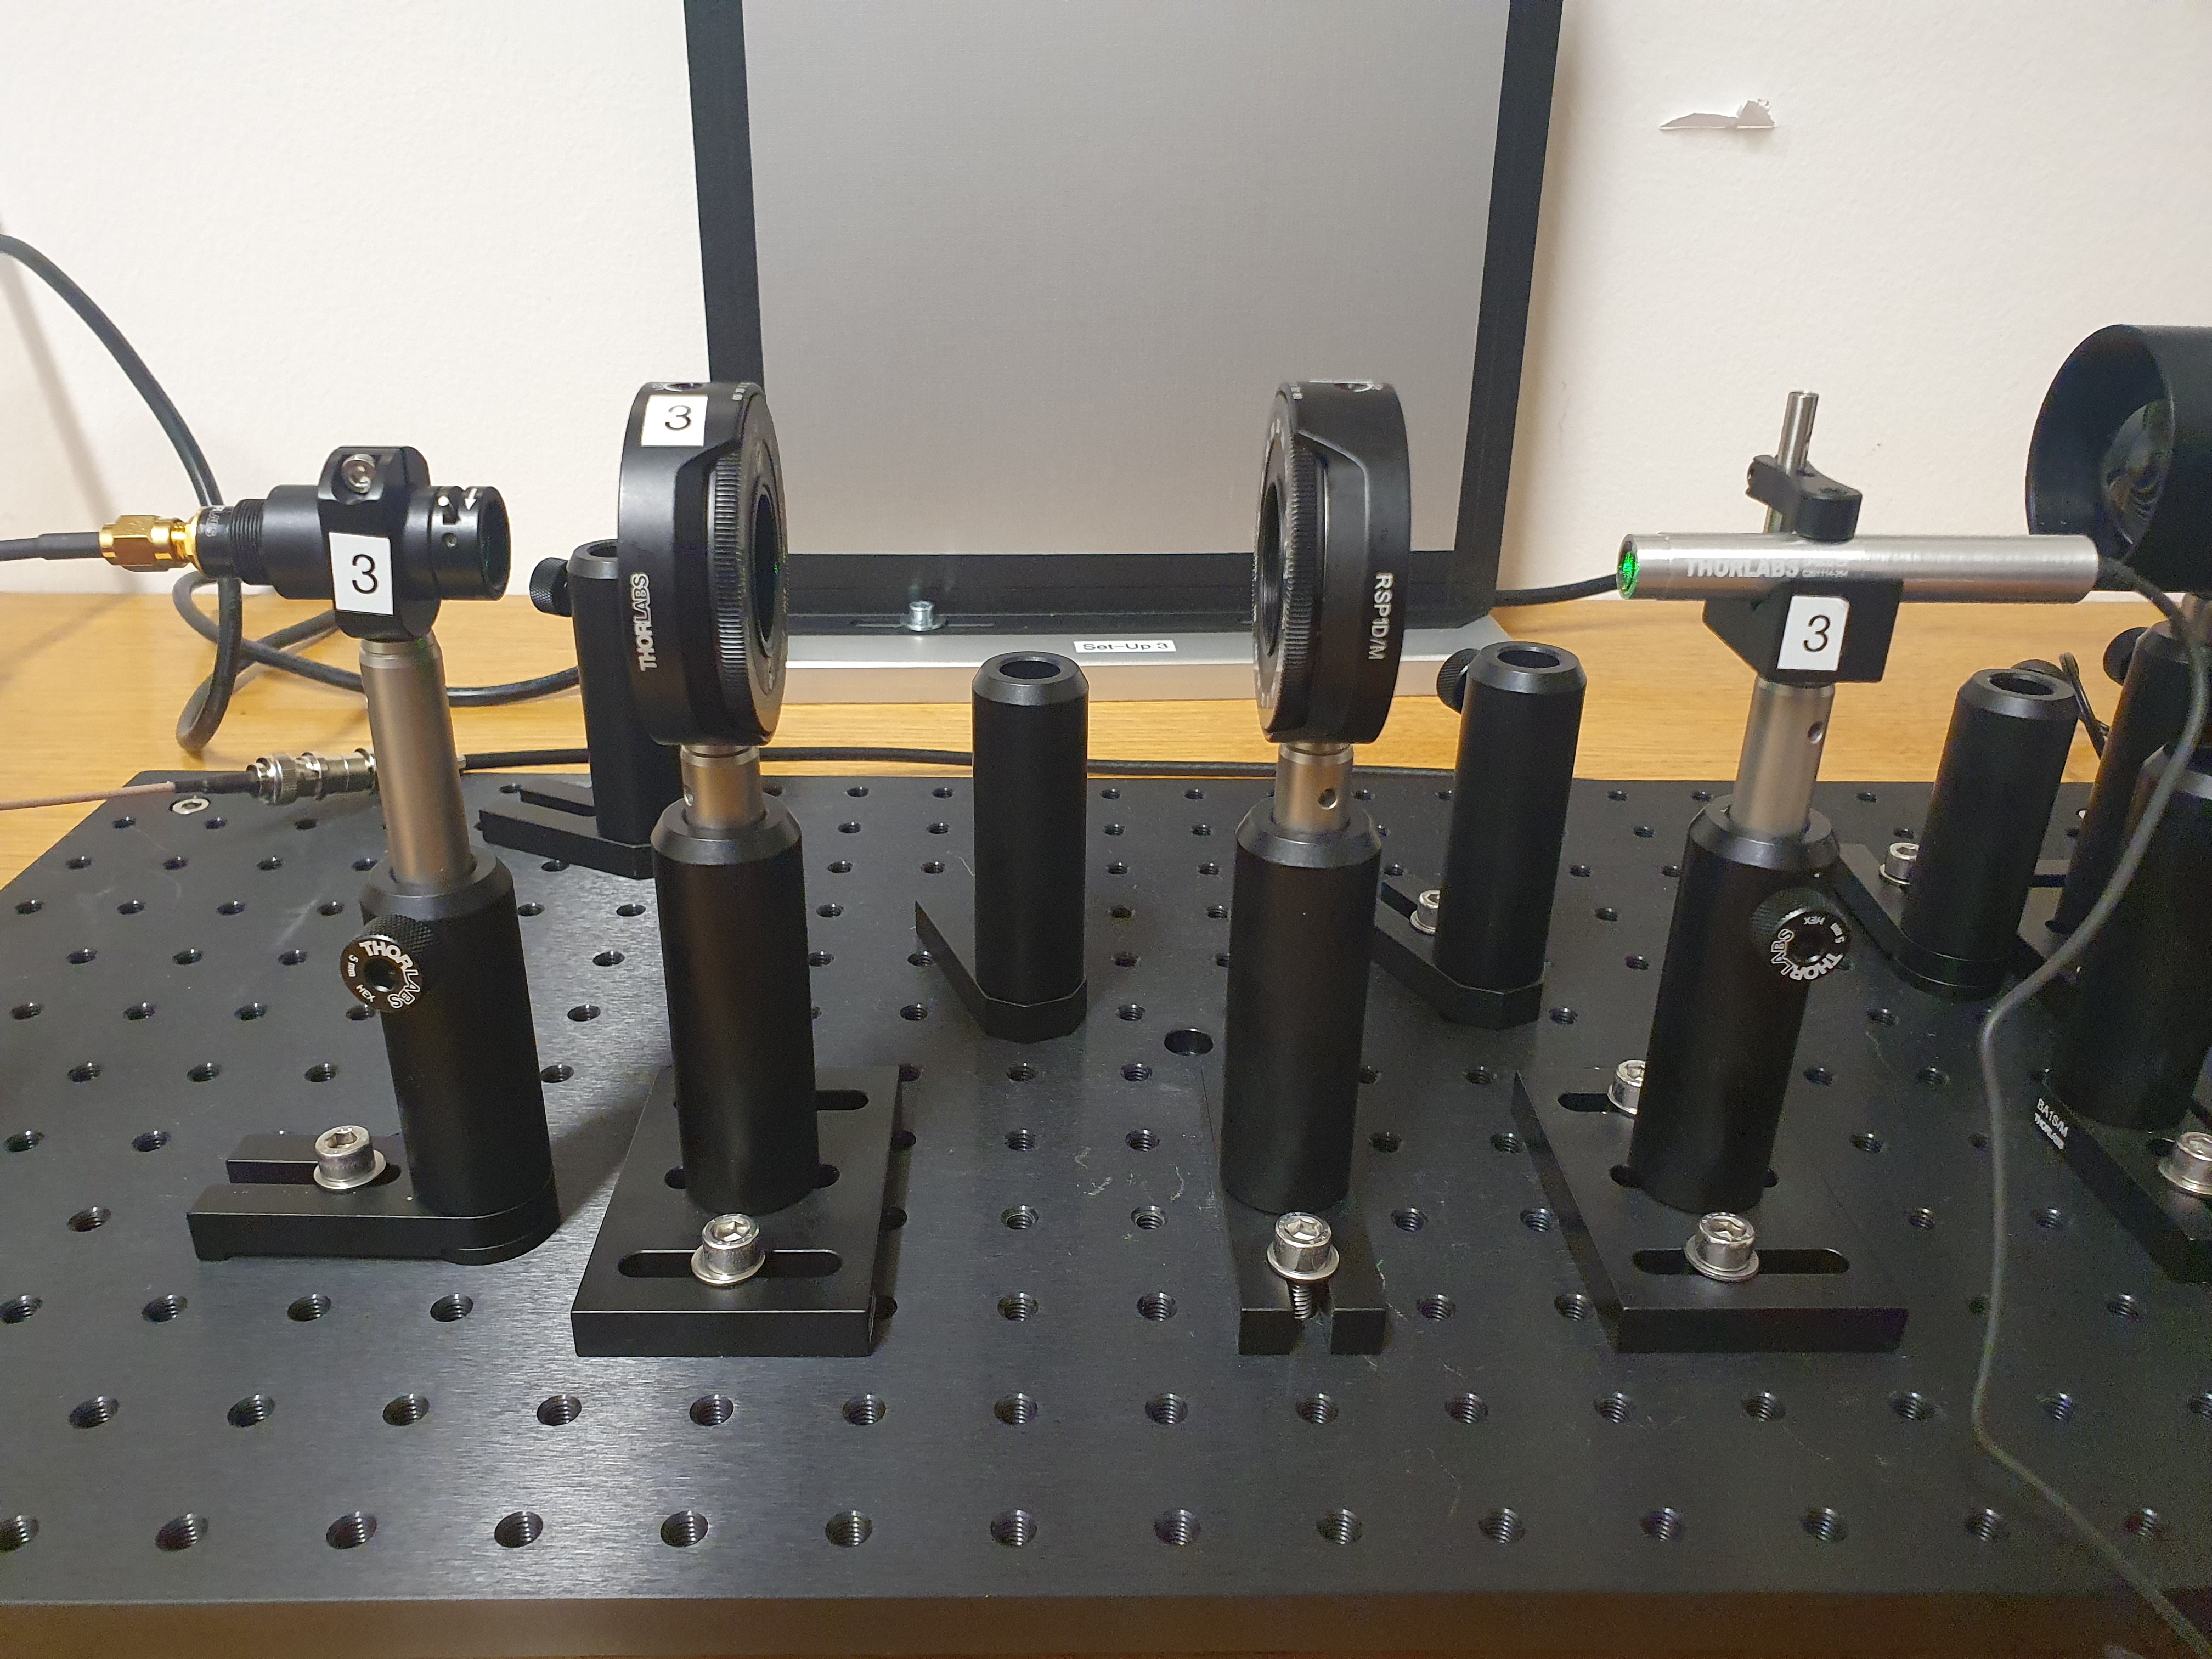
\includegraphics[width=0.6\linewidth]{nudes/aufbau mallus.jpg}
        \caption{Versuchsaufbau für den Beweis des Gesetzes von Malus}
        \label{fig:mallus aufbau}
    \end{figure}

\noindent
Ein Laser, welcher durch einen Polarisator verläuft, um linear Polarisiertes Licht zu erzeugen, trifft auf einen weiteren Polarisator, welcher immer um 10° gedreht wird. 
Hinter dem zweiten Polarisator befindet sich ein Photodetektor, welcher mit einem Voltmeter verbunden ist. 
\\
\\
Im zweiten Teil wird die konzentration einer Zuckerlösung ermittelt. Der Aufbau ist in etwa der selbe, nur dass zwischen die Polarisatoren eine Glas-Bassin mit Zuckerwasser kommt. 
Der Polarisator wird gedreht, bis kein Licht mehr durch fällt. Anschließend wird der Zuckertank entfernt und der Polarisator wird wieder soweit gedreht, bis kein Licht mehr durchfällt. 

\begin{figure}[H]
    \centering
    \includegraphics[width=0.6\linewidth, angle=-90]{nudes/zuckerlösung.jpg}
    \caption{Versuchsaufbau für den Zuckertank}
    \label{fig:zucker aufbau}
\end{figure}

\noindent
Der dritte Teil besteht aus einem Polarisator, welcher vor einem Handybildschirm steht, da dieser linear polarisiertes Licht ausstrahlt. 
Dazwischen stellt man verschiedene Objekte, wie zum Beispiel eine Plastikbox. Man erkennt verschiedene Wellenlängen, welche die Spannungen im Material sichtbar machen. 

\begin{figure}[H]
    \centering
    \includegraphics[width=0.6\linewidth, angle=-90]{nudes/schraubenschlüssel.jpg}
    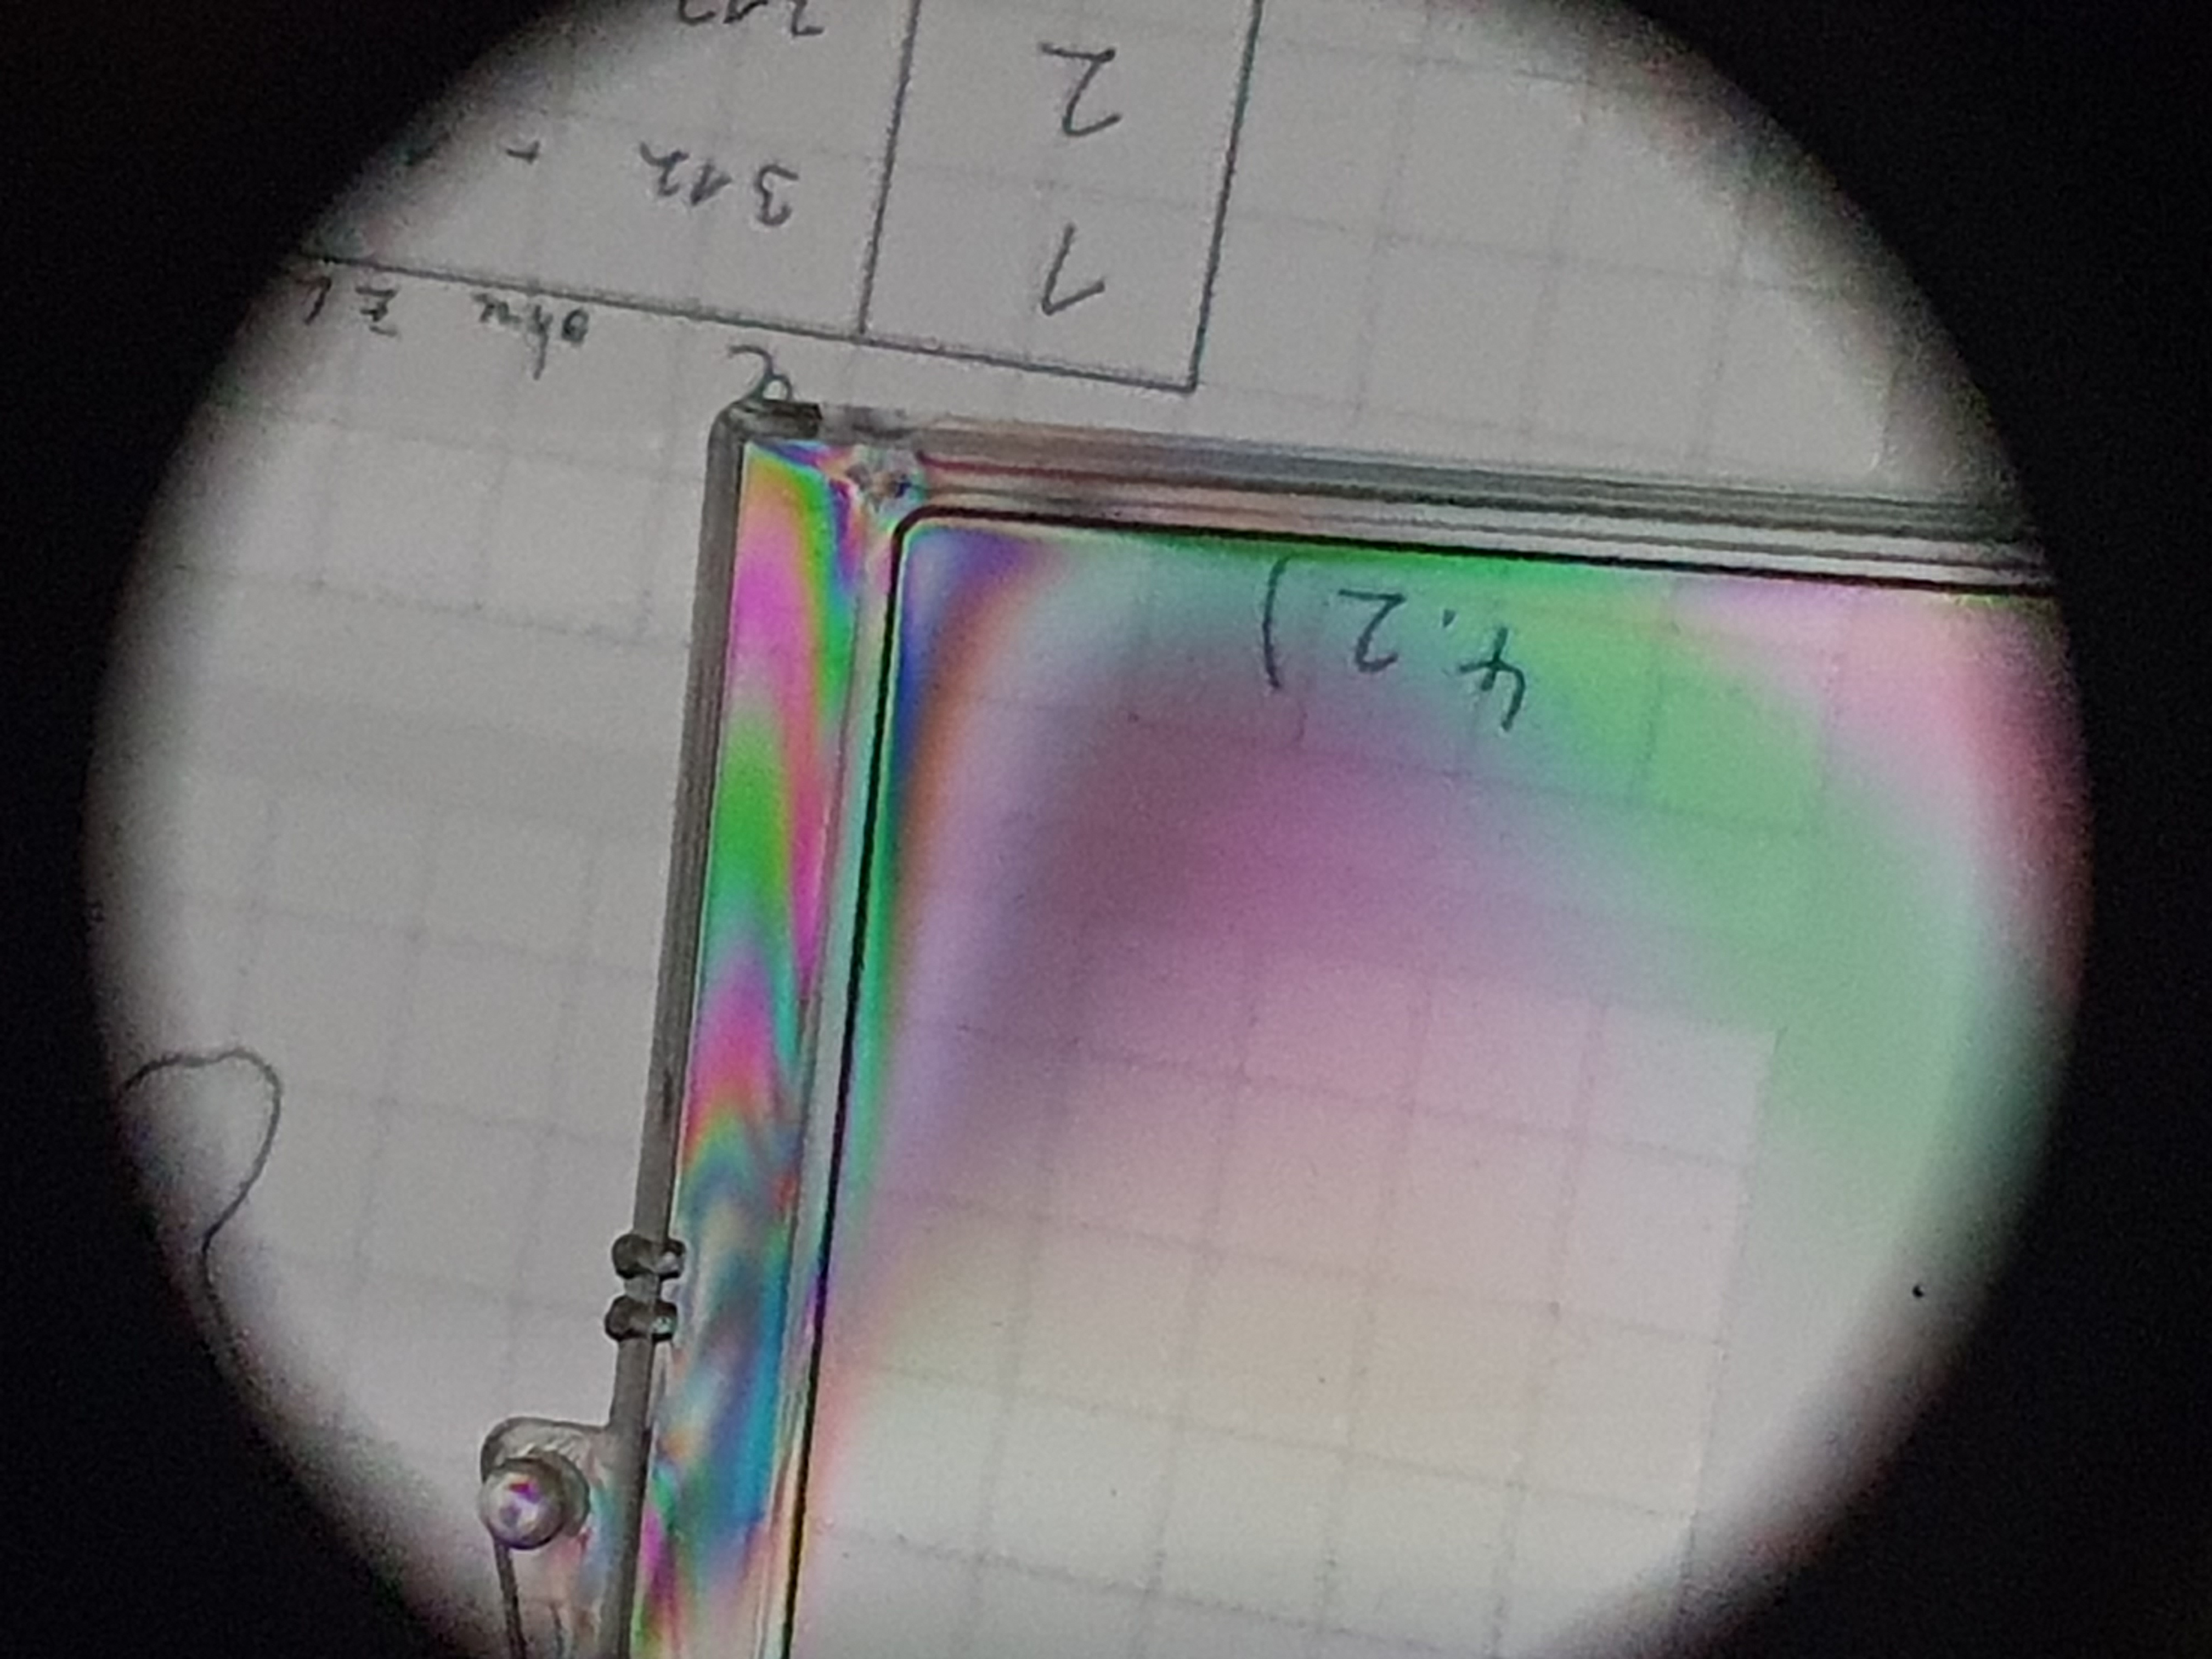
\includegraphics[width=0.6\linewidth, angle=-90]{nudes/plastikecke.jpg}
    \caption{Versuchsaufbau für die Spannungsdoppelbrechungen}
    \label{fig:Spannungsdoppelbrechungen aufbau}
\end{figure}

\noindent
Für die Bestimmung der Orientierung der Polarisatior Folien in einer 3D-Brille wird die Brille vor einen Polarisator gestellt. Hinter der Brille ist ein weiterer Polarisator und ein Photodetektor. 
Durch Messungen am Photodetektor in 10° Schritten wird die Polarisationsachse bestimmt. 
\\
Der Versuch ist für jedes Brillenglas einzeln zu machen. 

\begin{figure}[H]
    \centering
    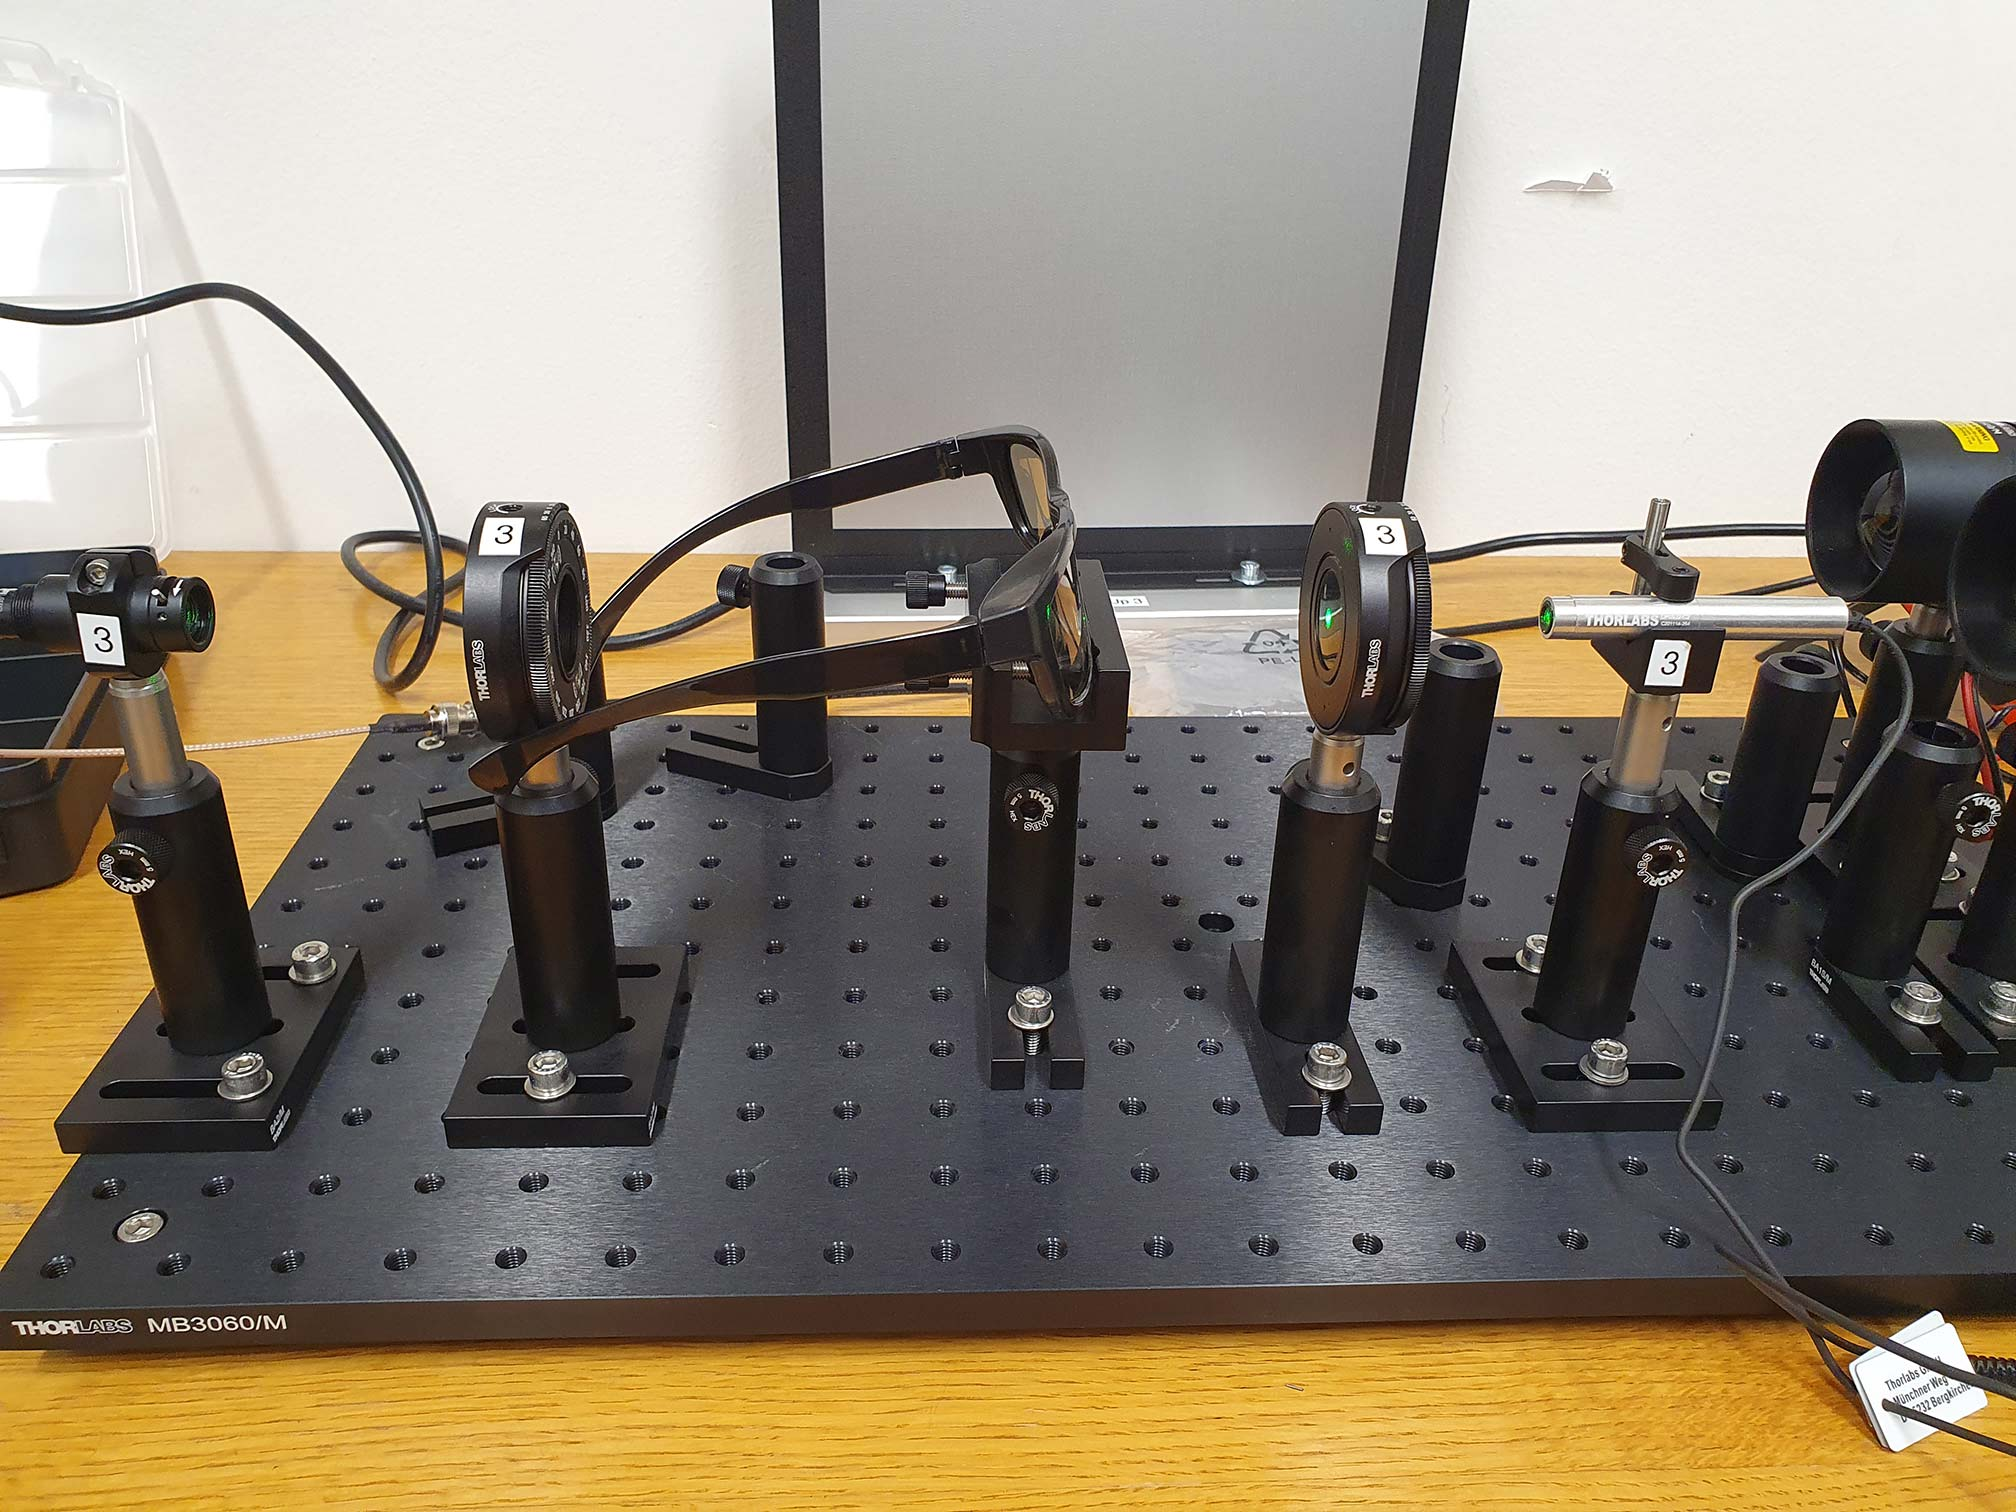
\includegraphics[width=0.6\linewidth]{nudes/3d-brille aufbau.jpg}
    \caption{Versuchsaufbau für die 3D-Brille}
    \label{fig:3D Brille aufbau}
\end{figure}

\noindent
Um nun ein 3D Bild zu erzeugen, benötigt es mehrere Schritte. 
Im ersten Schritt müssen die Polarisatoren auf die 3D-Brille abgestimmt werden.
Hierzu spannt man die Brille vor einen Laser und dreht den Polarisator hinter der Brille bis kein Licht mehr an der Leinwand ankommt. 
Ist dies der Fall dreht man den Polarisator um 90° weiter. Dies macht man für beide Brillen. 

\begin{figure}[H]
    \centering
    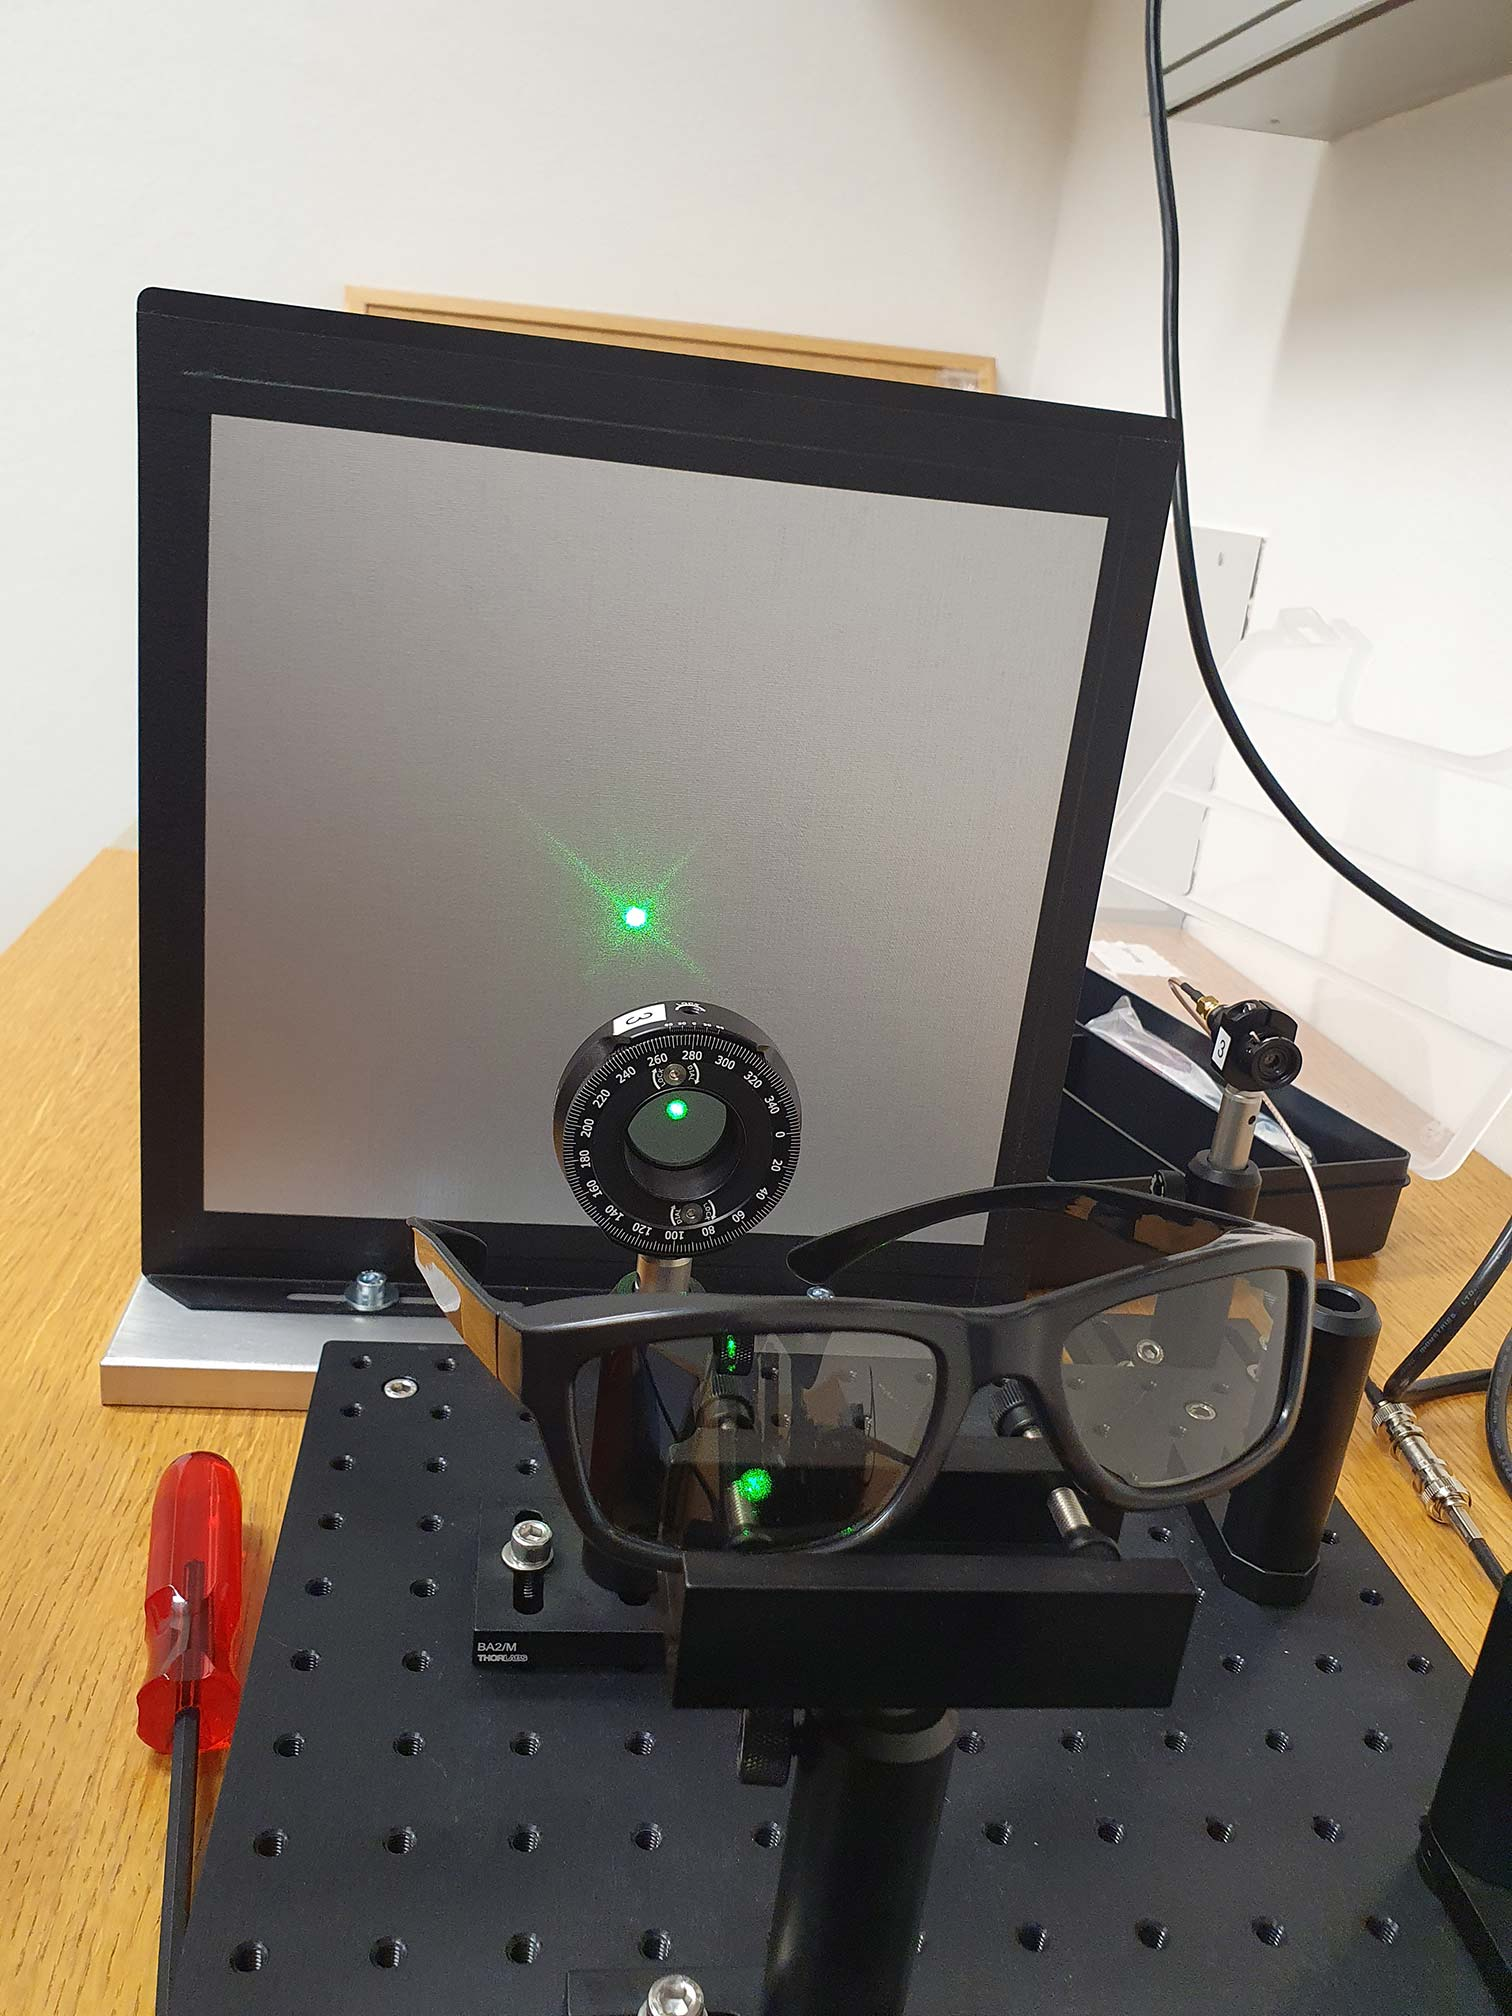
\includegraphics[width=0.6\linewidth, angle=-90]{nudes/brille rechts.jpg}
    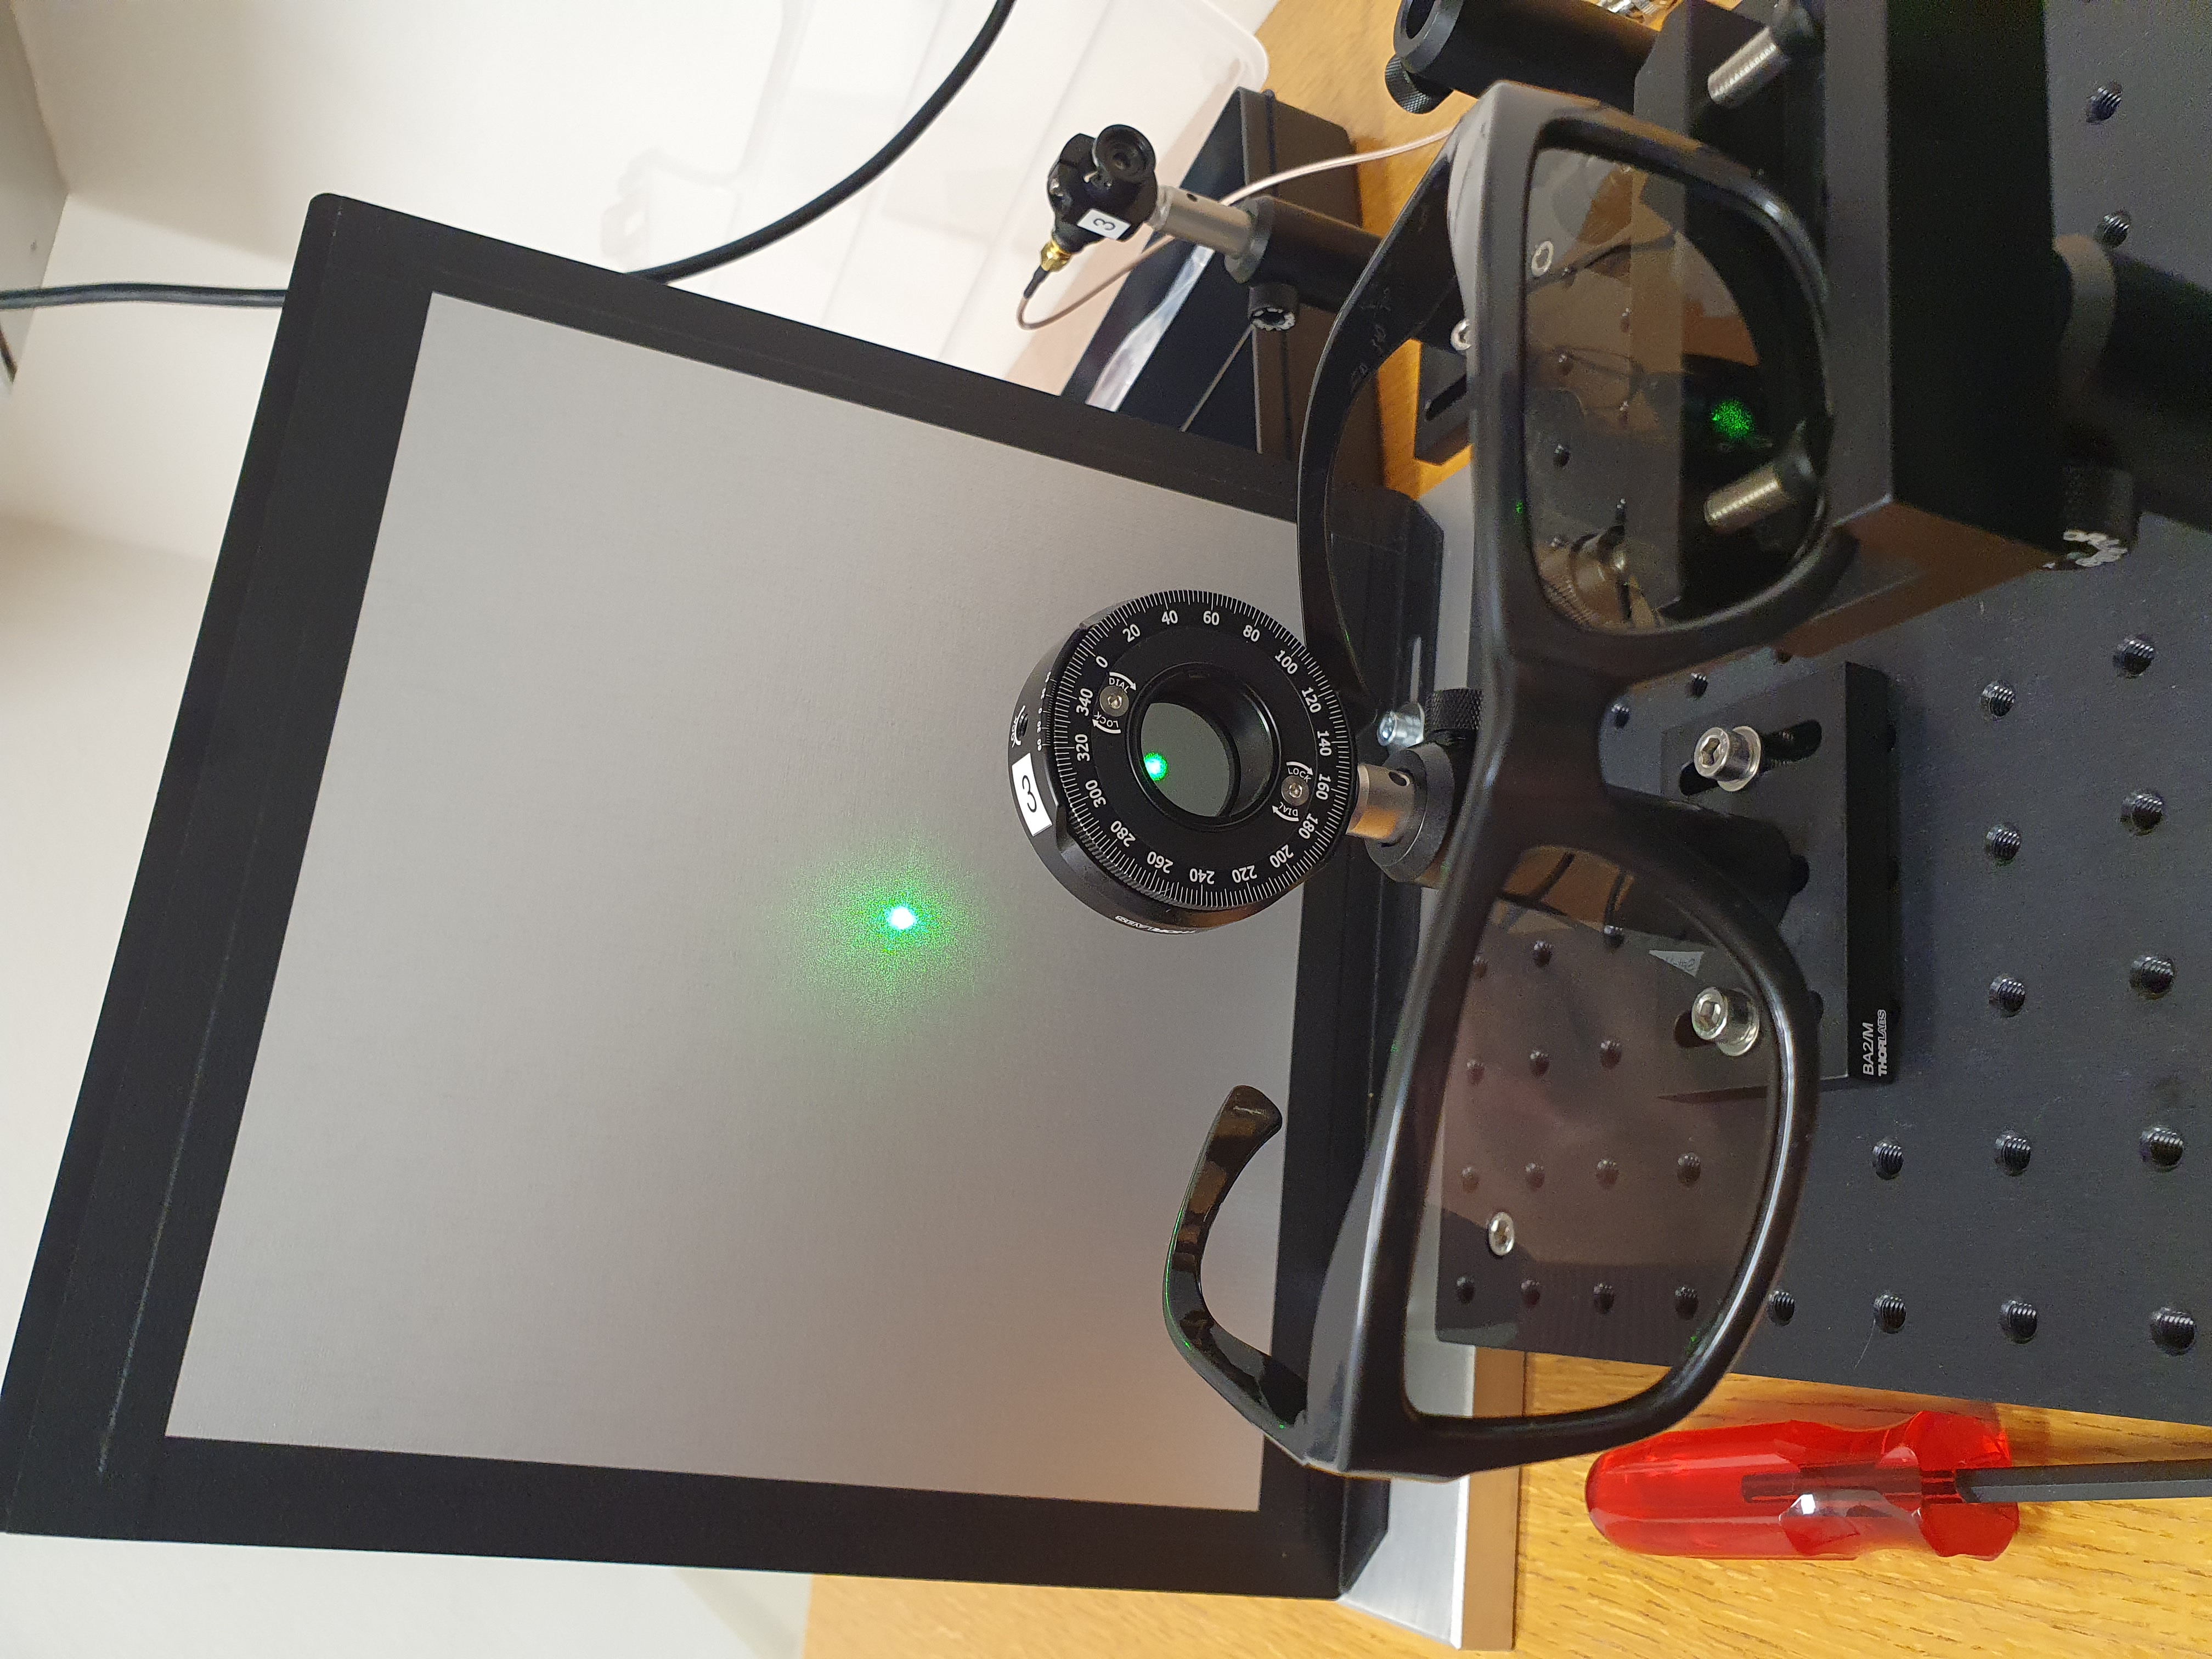
\includegraphics[width=0.6\linewidth, angle=-90]{nudes/brille links.jpg}
    \caption{Versuchsaufbau für das 3D-Kino, einstellen des Polarisators}
    \label{fig:3D Brille polarisator aufbau}
\end{figure}

\noindent
Für die Projektion stellt man die Dias vor die Lampen. Dahinter stellt man für jede Lampe eine Linse. 
Das Bild wird scharfgestellt und dann fügt man die Polarisatoren und die $\lambda/4$ Plättchen hinzu. 
Ist alles richtig aufgebaut, so kann man das Dia mit der 3D-Brille beobachten und es sollte ein 3D-Effekt auftreten. 

\begin{figure}[H]
    \centering
    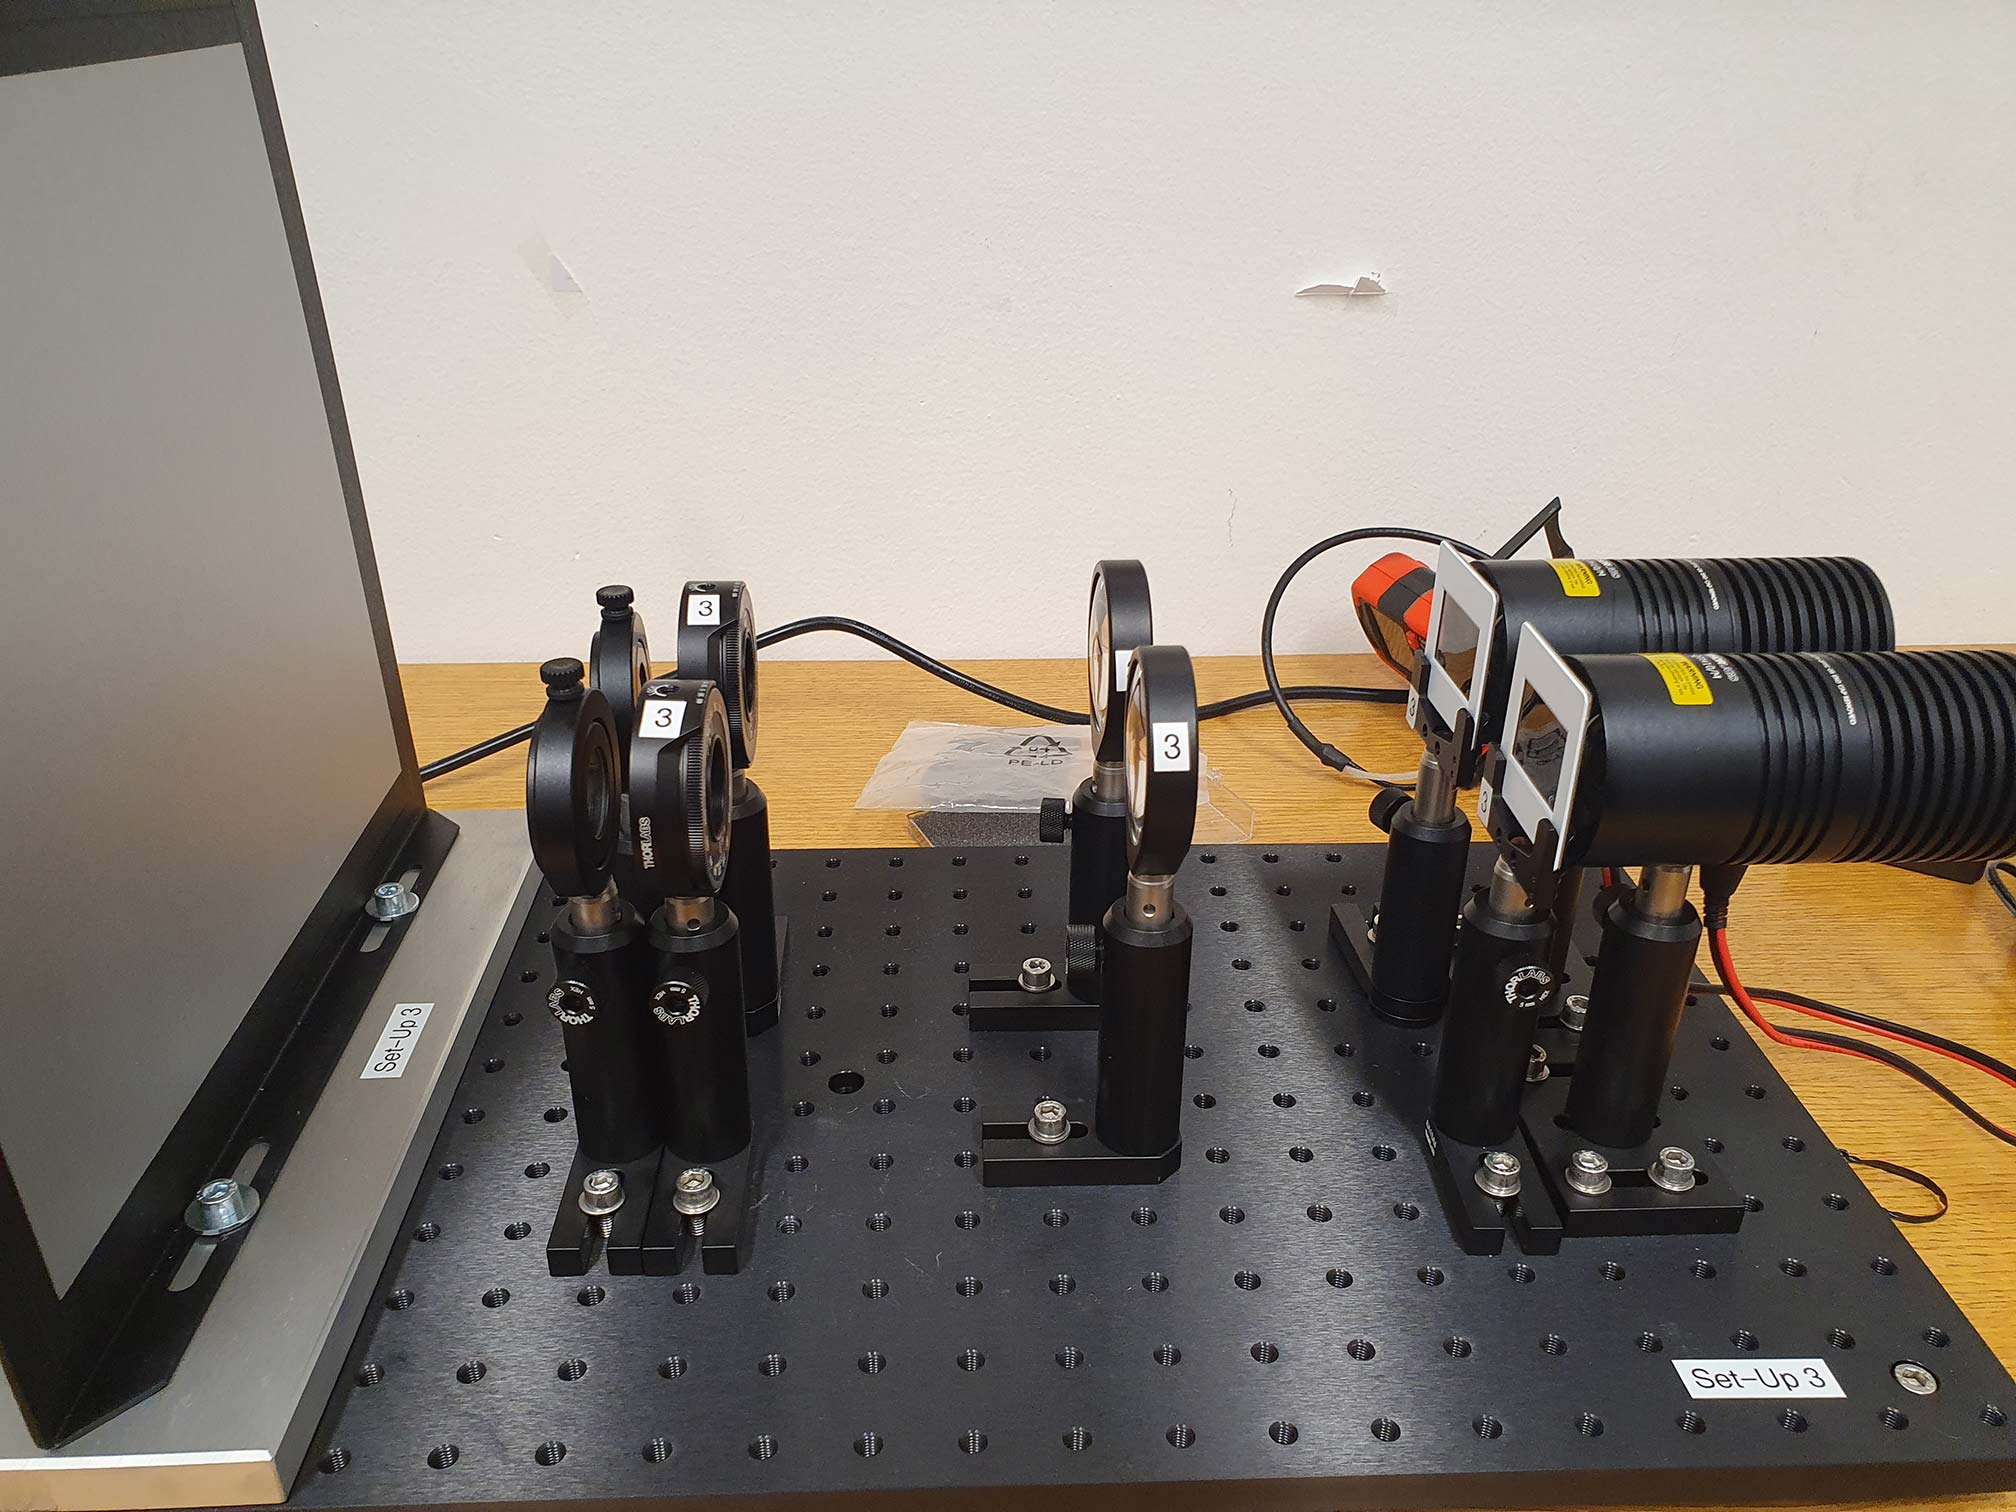
\includegraphics[width=0.6\linewidth]{nudes/3d kino aufbau hell.jpg}
    \caption{Versuchsaufbau für das 3D-Kino, anordnung der Optischen Bauteile}
    \label{fig:3D Kino aufbau}
\end{figure}

\begin{figure}[H]
    \centering
    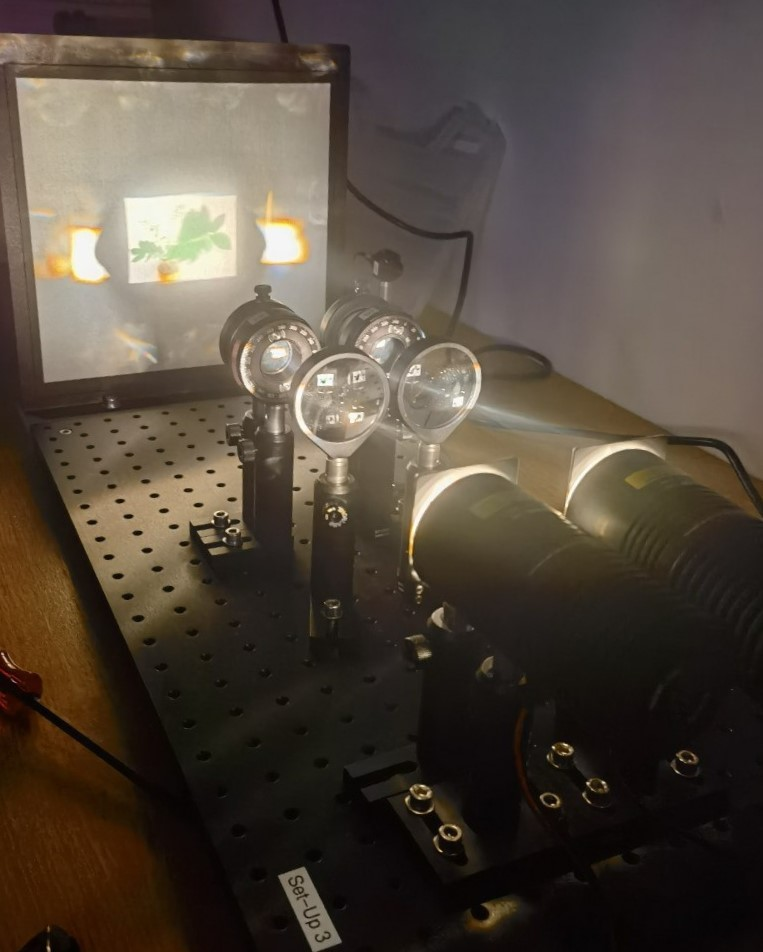
\includegraphics[width=0.6\linewidth]{nudes/3d kino aufbau.jpg}
    \caption{Versuchsaufbau für das 3D-Kino, 3D-Projektion}
    \label{fig:3D Kino projektion}
\end{figure}

\section{Geräteliste} %jo holt a listn ------------------------------

    \begin{table}[H]
        \centering
        \caption{Im Versuch verwendete Geräte und Utensilien.}
        \label{tab:geraete}
        \begin{tabular}{| l | l | l |}
            \hline
            Gerät   & Gerätenummer  & Unsicherheit \\
            \hline
            3D-Kino Setup 3 & Thorlabs MB3060/M & {n.a} \\
            Polarisatoren & Thorlabs PSP1D/M & $\pm 5 arcmin$\\
            Laser & Thorlabs CPS532-C2 & {n.a}\\
            Photodetektor & Thorlabs {n.a} & {n.a}\\
            Voltmeter & RSPro RS-12 & $\pm(0.5\% reading + 2 digits)V$ \cite{voltmeter} \\
            Plastikproben & {n.a} & {n.a} \\
            3D Brille & RealD & {n.a} \\
            $\lambda/4$ Plättchen & Thorlabs LM1-BM & {n.a} \\
            Projektoren & Thorlabs {n.a} & {n.a} \\
            Dias & {n.a} & {n.a} \\
            Rollmeter & {n.a} & $\pm 0.3mm$ \\
            \hline
        \end{tabular}
    \end{table}


\section{Versuchsdurchführung \& Messergebnisse} %nachvollziehbar und klar dargestellt ------------------------------
Für den ersten Teil wurde die Gradzahl des Polarisators auf den höchsten Wert gestellt, welcher in diesen Fall 240° betrug.
In 10° schritten wurden Messwerte aufgezeichnet. Da die Bogenminuten bei der Messung des Maximums auf 0 fielen, wurden sie nicht aufgeschrieben. 

\begin{table}[H]
    \centering
    \caption{Messdaten der Spannung $U$ des Multimeters.
    \\
    Dabei ist $U$ der gemessene Wert und $\bar{U}$ der Mittelwert, in der Tabelle jeweils das zweite $U$, da der Balken kaum sichtbar ist. }
    \label{tab:Messdaten Mallus}
    \begin{tabular}{| l | l | l | l | l | l |}
        \hline
        Winkel $\varphi$ [°] & $U$ [mv] & $\bar{U}$ [mV] & Winkel $\varphi$ [°] & $U$ [mv] & $\bar{U}$ [mV] \\
        \hline
        0    & 191 - 174 & 182,5  & 180   & 112 - 97  &104,5 \\
        10   & 213 - 199 & 206,0  & 190   & 151 - 132 &141,5 \\
        20   & 208 - 219 & 213,0  & 200   & 174 - 155 &164,5 \\
        30   & 212 - 224 & 218,0  & 210   & 186 - 169 &177,5 \\
        40   & 225 - 214 & 219,5  & 220   & 196 - 181 &188,5 \\
        50   & 224 - 213 & 218,5  & 230   & 205 - 190 &197,5 \\
        60   & 212 - 198 & 205,0  & 240   & 206 - 192 &199,0 \\
        70   & 181 - 197 & 189,0  & 250   & 183 - 198 &190,5 \\
        80   & 173 - 153 & 163,0  & 260   & 178 - 160 &169,0 \\
        90   & 136 - 117 & 126,5  & 270   & 144 - 125 &134,5 \\
        100  & 79 - 67   &  73,0  & 280   & 83 - 97   & 90,0  \\
        110  & 38 - 32   &  35,0  & 290   & 54 - 46   & 50,0  \\
        120  & 15 - 12   &  13,5  & 300   & 21 - 18   & 19,5  \\
        130  & 2 - 1     &   1,5  & 310   & 1 - 2     &  1,5   \\
        140  & 3 - 2     &   2,5  & 320   & 5 - 4     &  4,5   \\
        150  & 15 - 18   &  16,5  & 330   & 25 - 29   & 27,0  \\
        160  & 40 - 47   &  43,5  & 340   & 60 - 70   & 65,0  \\
        170  & 81 - 71   &  76,0  & 350   & 115 - 134 &124,5 \\
        \hline
    \end{tabular}
\end{table}

\noindent
Im zweiten Teil wurden die Winkel mit und ohne Zuckerlösung insgesamt fünf mal gemessen. Die Messung erfolgte, wenn kein Licht mehr durch den Polarisator fiel. 
\\
Die Länge des Zuckerbassins beträgt $(21.5 \pm 0.1)cm$, der Winkel $\varphi_0$ beträgt laut Skriptum $\varphi_0 = 6.65$° \cite{teachcenter2}. 

\begin{table}[H]
    \centering
    \caption{Winkel $\varphi$ mit und ohne Zuckerlösung}
    \label{tab:Messdaten Zuckerlösung}
    \begin{tabular}{| l | l | l | l | l |}
        \hline
        Nr. & Winkel ohne ZL $\varphi$ [°] & U [mv] & Winkel mit ZL $\varphi$ [°] & U [mv] \\
        \hline
        1   & 312 + 10  & 0.5   & 336 + 35 & 1.0 - 1.2 \\
        2   & 312 + 30  & 0.5   & 334 + 20 & 0.9 - 1.0 \\
        3   & 312 + 35  & 0.5   & 338 + 10 & 0.8 - 0.7 \\
        4   & 312 + 15  & 0.5   & 336 + 35 & 1.0 - 0.9 \\
        5   & 312 + 15  & 0.5   & 336 + 40 & 1.0 - 0.9 \\
        \hline
    \end{tabular}
\end{table}

\noindent
Im dritten Teil gab es keine Messwerte, welche aufgenommen werden hätten können. \\
\\
Im vierten Teil wird für eine 3D Brille die Polarisation bestimmt. Dabei ist zu beachten, jedes Auge einzeln zu vermessen. 
Da die Bogenminuten bei der Messung auf 0 fielen, wurden sie nicht aufgeschrieben. 
\begin{table}[H]
    \centering
    \caption{Auge 1 (rechts)}
    \label{tab:Messdaten Auge rechts}
    \begin{tabular}{| l | l | l | l |}
        \hline
        Winkel $\varphi$ [°] & $U$ [mv] & Winkel $\varphi$ [°] & $U$ [mv] \\
        \hline
        0    & 263  & 180   & 260  \\
        10   & 251  & 190   & 276  \\
        20   & 216  & 200   & 251  \\
        30   & 232  & 210   & 236  \\
        40   & 198  & 220   & 212  \\
        50   & 105  & 230   & 90  \\
        60   & 12   & 240   & 19  \\
        70   & 4    & 250   & 4  \\
        80   & 72   & 260   & 83  \\
        90   & 191  & 270   & 191  \\
        100  & 235  & 280   & 201  \\
        110  & 267  & 290   & 239  \\
        120  & 274  & 300   & 270  \\
        130  & 273  & 310   & 273  \\
        140  & 281  & 320   & 276  \\
        150  & 282  & 330   & 278  \\
        160 max  & 287  & 340   & 274  \\
        170  & 278  & 350   & 273  \\
        \hline
    \end{tabular}
\end{table}

\begin{table}[H]
    \centering
    \caption{Auge 2 (links)}
    \label{tab:Messdaten Auge links}
    \begin{tabular}{| l | l | l | l |}
        \hline
        Winkel $\varphi$ [°] & $U$ [mv] & Winkel $\varphi$ [°] & $U$ [mv] \\
        \hline
        0    & 247  & 180   & 248  \\
        10   & 228  & 190   & 249  \\
        20   & 192  & 200   & 243  \\
        30   & 203  & 210   & 200  \\
        40   & 151  & 220   & 186  \\
        50   & 71   & 230   & 67   \\
        60   & 10   & 240   & 15   \\
        70   & 1    & 250   & 2    \\
        80   & 35   & 260   & 36   \\
        90   & 122  & 270   & 150  \\
        100  & 202  & 280   & 154  \\
        110  & 247  & 290   & 198  \\
        120  & 255  & 300   & 244  \\
        130  & 256  & 310   & 259  \\
        140  & 264  & 320   & 253  \\
        150  & 267  & 330   & 259  \\
        160 max & 272  & 340   & 259  \\
        170  & 267  & 350   & 257  \\
        \hline
    \end{tabular}
\end{table}


\section{Auswertung und Unsicherheitsanalyse} %Nicht nur zahlen angeben ------------------------------
In der Auswertung werden zur erhöhten Genauigkeit durchgehend ungerundete Werte bis zu den Endergebnissen verwendet und nur zur Darstellung gerundet. \\
Zur Berechnung der Unsicherheiten wird die Größtunsicherheitsmethode verwendet.

Im ersten Teil gilt es das Gesetz von Malus zu beweisen. 
Aus den Messdaten der Tabelle \ref{tab:Messdaten Mallus} wird ein Graph erzeugt. 

\section{Diskussion} %diskussion der Unsicherheiten und Ergebnisse und evtl. verlgeich mit Literatur ------------------------------


\section{Zusammenfassung} %klare, übersichtliche vollständige beantwortung der Aufgabenstellung ------------------------------



\printbibliography[heading=bibintoc]
\end{document}
